\documentclass[10pt,twocolumn,letterpaper]{article}

\usepackage[utf8]{inputenc}
\usepackage[margin=0.8in]{geometry}
\usepackage{graphicx}
\usepackage{booktabs}
\usepackage{amsmath}
\usepackage{hyperref}

% Numbers in the text come from results/macros.tex, which scripts/train_models.py writes.
% If it is missing (no run yet), every number prints as "??".
\IfFileExists{results/macros.tex}{\newcommand{\nTest}{1441}
\newcommand{\majorityAcc}{0.676}
\newcommand{\smokeTest}{0}
\newcommand{\hardware}{Apple M5, 16 GB}
\newcommand{\resnetTestAcc}{0.773}
\newcommand{\resnetTestBacc}{0.706}
\newcommand{\resnetTestBaccCI}{[0.648, 0.764]}
\newcommand{\resnetTestFone}{0.607}
\newcommand{\resnetMelRecall}{0.493}
\newcommand{\resnetBestEpoch}{4}
\newcommand{\resnetEpochs}{5}
\newcommand{\resnetMinPerEpoch}{3.2}
\newcommand{\vitTestAcc}{0.745}
\newcommand{\vitTestBacc}{0.728}
\newcommand{\vitTestBaccCI}{[0.670, 0.784]}
\newcommand{\vitTestFone}{0.610}
\newcommand{\vitMelRecall}{0.616}
\newcommand{\vitBestEpoch}{3}
\newcommand{\vitEpochs}{5}
\newcommand{\vitMinPerEpoch}{8.2}
\newcommand{\nTrain}{7126}
\newcommand{\nVal}{1448}
\newcommand{\nImages}{10015}
\newcommand{\nLesions}{7470}
\newcommand{\baccDiff}{-0.022}
\newcommand{\baccDiffCI}{[-0.088, +0.048]}
}{}
\providecommand{\smokeTest}{0}
\newcommand{\PH}{\textbf{??}}
\providecommand{\nImages}{\PH}\providecommand{\nLesions}{\PH}
\providecommand{\nTrain}{\PH}\providecommand{\nVal}{\PH}\providecommand{\nTest}{\PH}
\providecommand{\majorityAcc}{\PH}\providecommand{\hardware}{\PH}
\providecommand{\resnetTestAcc}{\PH}\providecommand{\resnetTestBacc}{\PH}\providecommand{\resnetTestBaccCI}{\PH}
\providecommand{\resnetTestFone}{\PH}\providecommand{\resnetMelRecall}{\PH}\providecommand{\resnetBestEpoch}{\PH}
\providecommand{\resnetEpochs}{\PH}\providecommand{\resnetMinPerEpoch}{\PH}
\providecommand{\vitTestAcc}{\PH}\providecommand{\vitTestBacc}{\PH}\providecommand{\vitTestBaccCI}{\PH}
\providecommand{\vitTestFone}{\PH}\providecommand{\vitMelRecall}{\PH}\providecommand{\vitBestEpoch}{\PH}
\providecommand{\vitEpochs}{\PH}\providecommand{\vitMinPerEpoch}{\PH}
\providecommand{\baccDiff}{\PH}\providecommand{\baccDiffCI}{\PH}

\title{Fine-Tuning ResNet-50 and ViT-Base for Seven-Class Skin Lesion Classification on HAM10000 with a Laptop GPU}
\author{Yafattah Rayane}
\date{January 2026, revised November 2026\ifnum\smokeTest=1\\[6pt]\fbox{\textbf{SMOKE TEST: NOT REAL RESULTS}}\fi}

\begin{document}

\maketitle

\begin{abstract}
I compare two ImageNet-pretrained backbones, ResNet-50~\cite{he2016deep} and ViT-Base/16~\cite{dosovitskiy2021image}, fine-tuned for seven-class classification of dermatoscopic images from HAM10000~\cite{tschandl2018ham10000}.
Images are split into training, validation and test sets at the lesion level, so that no lesion contributes images to more than one set.
Both models are trained for a few epochs on a MacBook Air GPU (\hardware; PyTorch MPS backend), with class-weighted cross-entropy and data augmentation to counter the strong class imbalance.
On the held-out test set ($n=\nTest$), ResNet-50 reaches a balanced accuracy of \resnetTestBacc{} (95\% bootstrap CI \resnetTestBaccCI) and ViT-Base \vitTestBacc{} (\vitTestBaccCI); always predicting the majority class gives 0.143.
The difference between the two models (\baccDiff{}, 95\% CI \baccDiffCI) is within test-set noise, while ResNet-50 trains about 2.6 times faster per epoch.
Both models remain weak on melanoma, with recall of \resnetMelRecall{} and \vitMelRecall{}.
These are results from one training run, one random seed and one data split, and are not a clinical evaluation.
\end{abstract}

\section{Introduction}
Automated classification of dermatoscopic images is a well-studied problem; melanoma in particular benefits from early detection.
Convolutional networks such as ResNet-50~\cite{he2016deep} build in locality and translation equivariance, while Vision Transformers~\cite{dosovitskiy2021image} model relations between image patches with self-attention and typically rely more on large-scale pre-training.

This project asks a narrow, practical question: with ImageNet pre-training, a short fine-tuning budget and a consumer laptop (MacBook Air, \hardware, PyTorch MPS backend), how do the two architectures compare on HAM10000~\cite{tschandl2018ham10000} when evaluated on lesions they have not seen?
The emphasis is on a sound evaluation protocol (lesion-level split, imbalance-aware metrics, a test set touched once) rather than on reaching state-of-the-art numbers.

\paragraph{Revision note.}
An earlier version of this report (January 2026) trained each model for one epoch on all 10,015 images on an Apple M4 machine and reported only the training loss, which does not measure generalisation; its supplementary heat-map was a placeholder graphic, not computed from a model.
Those results and that figure have been removed.
All numbers below come from \texttt{scripts/train\_models.py} and are written into this document automatically from its output files.

\section{Method}

\subsection{Data and split}
HAM10000~\cite{tschandl2018ham10000} contains \nImages{} dermatoscopic images of \nLesions{} distinct lesions in seven diagnostic classes (akiec, bcc, bkl, df, mel, nv, vasc).
Many lesions were photographed more than once, so a random image-level split would place near-duplicate images of the same lesion in both training and test sets and inflate test scores.
I therefore split by \texttt{lesion\_id} with scikit-learn's \texttt{StratifiedGroupKFold}, stratified on diagnosis, into roughly 70/15/15\% training, validation and test sets (\nTrain/\nVal/\nTest{} images; Table~\ref{tab:split}).
The split is saved to \texttt{splits/ham10000\_split.csv} and reused by every script.
The classes are highly imbalanced: melanocytic nevi (nv) make up about two thirds of the images, while dermatofibroma (df) and vascular lesions (vasc) each make up under 2\%.

\begin{table}[h]
\centering
\caption{Images per class in each split (lesion-level split).}
\label{tab:split}
\IfFileExists{results/split_table.tex}{\begin{tabular}{@{}lccc@{}}
\toprule
Class & Train & Val & Test \\ \midrule
akiec & 233 & 60 & 34 \\
bcc & 354 & 71 & 89 \\
bkl & 790 & 141 & 168 \\
df & 91 & 15 & 9 \\
mel & 779 & 188 & 146 \\
nv & 4779 & 952 & 974 \\
vasc & 100 & 21 & 21 \\
\midrule
Total & 7126 & 1448 & 1441 \\
\bottomrule
\end{tabular}
}{\textit{Generated by train\_models.py.}}
\end{table}

\subsection{Models and training}
ResNet-50 uses torchvision's ImageNet-1k weights (\texttt{IMAGENET1K\_V2}) with the final layer replaced by a 7-way linear layer.
ViT-Base/16 uses the Hugging Face \texttt{google/vit-base-patch16-224} checkpoint
with a new 7-way classification head.
Images are resized to $224\times224$ and normalised with each checkpoint's own mean and standard deviation.

Training augmentation is random resized cropping (scale 0.7--1.0), horizontal and vertical flips, rotation up to $20^\circ$ and mild colour jitter; dermatoscopic images have no canonical orientation, so these transforms preserve the label.
To counter imbalance, the cross-entropy loss is weighted per class by the inverse of its training-set frequency.

Both models are fine-tuned end to end with AdamW (weight decay 0.05), a cosine learning-rate schedule, batch size 32 and a learning rate of $10^{-4}$ for ResNet-50 and $2\times10^{-5}$ for ViT-Base, for \resnetEpochs{} epochs.
After each epoch I compute balanced accuracy on the validation set and keep the best checkpoint.
The test set is evaluated once, with that checkpoint.
No other hyperparameters were tuned.
Training ran on a MacBook Air (\hardware) with PyTorch's MPS backend.

\subsection{Metrics}
Because always predicting nv already gives about 67\% accuracy, plain accuracy says little here.
I report balanced accuracy (the mean of per-class recall), macro-averaged F1 and per-class recall, alongside accuracy.
95\% confidence intervals are percentile bootstrap intervals over test images (2,000 resamples); the difference between the two models uses a paired bootstrap on the same resampled images.
These intervals reflect test-set sampling only, not variation between training runs.

\section{Results}
\label{sec:results}

\begin{table}[h]
\centering
\caption{Test-set results of the checkpoint with the best validation balanced accuracy ($n=\nTest$ images). Bal.\ acc.\ = balanced accuracy; min/ep.\ = mean training time per epoch on the laptop GPU.}
\label{tab:results}
\resizebox{\linewidth}{!}{%
\IfFileExists{results/results_table.tex}{\begin{tabular}{@{}lcccc@{}}
\toprule
Model & Test acc. & Test bal. acc. [95\% CI] & Macro F1 & min/ep. \\ \midrule
Majority (nv) & 0.676 & 0.143 & -- & -- \\
ResNet-50 & 0.773 & 0.706 [0.648, 0.764] & 0.607 & 3.2 \\
ViT-Base/16 & 0.745 & 0.728 [0.670, 0.784] & 0.610 & 8.2 \\
\bottomrule
\end{tabular}
}{\textit{Generated by train\_models.py.}}}
\end{table}

\begin{table}[h]
\centering
\caption{Per-class recall on the test set; $n$ is the number of test images per class.}
\label{tab:perclass}
\IfFileExists{results/per_class_recall.tex}{\begin{tabular}{@{}lccc@{}}
\toprule
Class & $n$ & ResNet-50 & ViT-Base/16 \\ \midrule
akiec & 34 & 0.765 & 0.765 \\
bcc & 89 & 0.820 & 0.674 \\
bkl & 168 & 0.500 & 0.583 \\
df & 9 & 0.556 & 0.667 \\
mel & 146 & 0.493 & 0.616 \\
nv & 974 & 0.856 & 0.793 \\
vasc & 21 & 0.952 & 1.000 \\
\bottomrule
\end{tabular}
}{\textit{Generated by train\_models.py.}}
\end{table}

Table~\ref{tab:results} summarises test performance.
ResNet-50 reaches a balanced accuracy of \resnetTestBacc{} \resnetTestBaccCI{} and accuracy \resnetTestAcc{}; ViT-Base reaches \vitTestBacc{} \vitTestBaccCI{} and \vitTestAcc{}.
The paired bootstrap difference in balanced accuracy (ResNet-50 minus ViT-Base) is \baccDiff{}, 95\% CI \baccDiffCI{}; if this interval contains zero, the run does not show a reliable difference between the two architectures.
Melanoma recall is \resnetMelRecall{} for ResNet-50 and \vitMelRecall{} for ViT-Base.
The best validation epoch was \resnetBestEpoch{} of \resnetEpochs{} for ResNet-50 and \vitBestEpoch{} of \vitEpochs{} for ViT-Base.
One training epoch took on average \resnetMinPerEpoch{} min for ResNet-50 and \vitMinPerEpoch{} min for ViT-Base.

% The numbers in this paragraph are from the 19 Nov 2026 run (results/*_metrics.json); update them if you rerun.
In balanced accuracy both models are far above the majority-class baseline, but in plain accuracy they are only 7--10 points above it: the class-weighted loss trades accuracy on the dominant nv class for recall on the rare classes.
Figure~\ref{fig:cm} shows where the errors are.
Melanoma is the main weakness of both models.
ViT-Base recalls more melanomas than ResNet-50 (90 vs.\ 72 of 146) but also labels about twice as many nevi as melanoma (143 vs.\ 72), so its melanoma precision is lower (0.34 vs.\ 0.42).
Many benign keratoses (bkl) are predicted as actinic keratoses (akiec), which gives akiec a low precision (0.25 and 0.33) despite a recall of 0.77 for both models.
Dermatofibroma (df) has only 9 test images, so its recall is not a reliable estimate.
Validation balanced accuracy at the selected epoch (0.722 and 0.750) is slightly higher than on the test set, as expected when the epoch is chosen on validation data.
Validation loss was still decreasing at epoch 5 for both models, so a longer schedule might help; this was not tested.

\begin{figure*}[t]
\centering
\IfFileExists{results/resnet50_confusion_test.png}{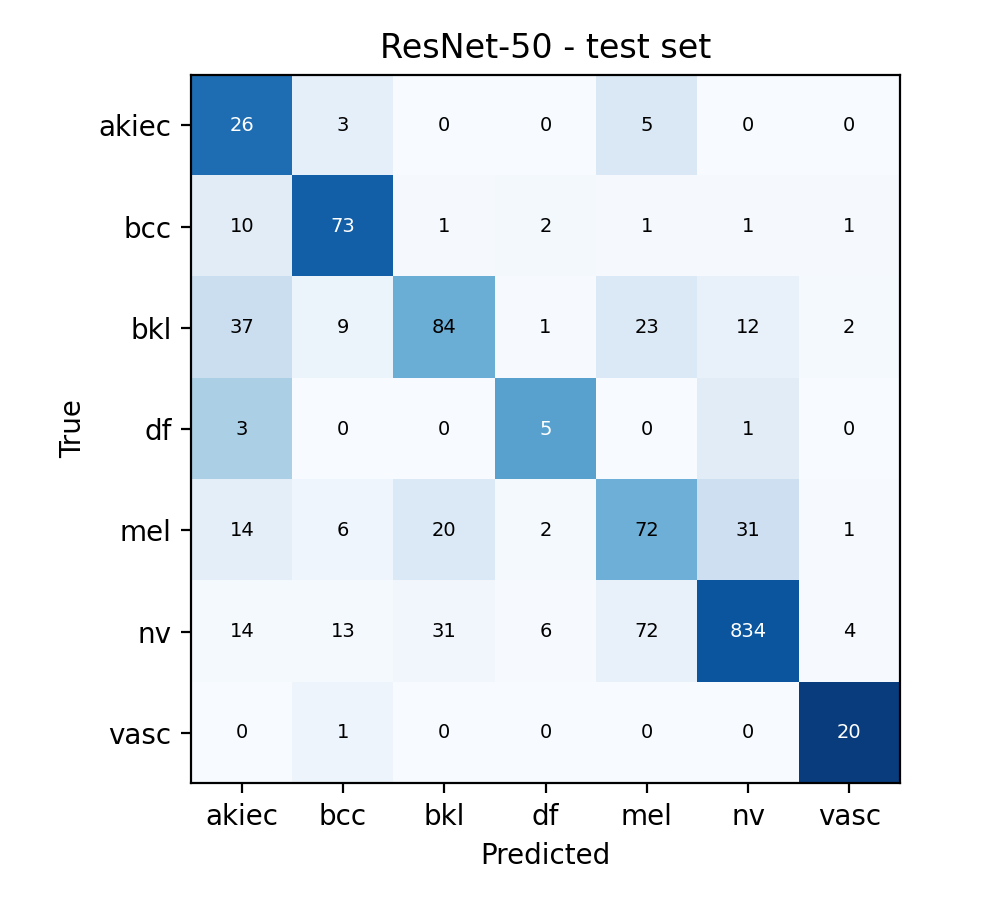
\includegraphics[width=0.42\textwidth]{results/resnet50_confusion_test.png}}{}%
\IfFileExists{results/vit_confusion_test.png}{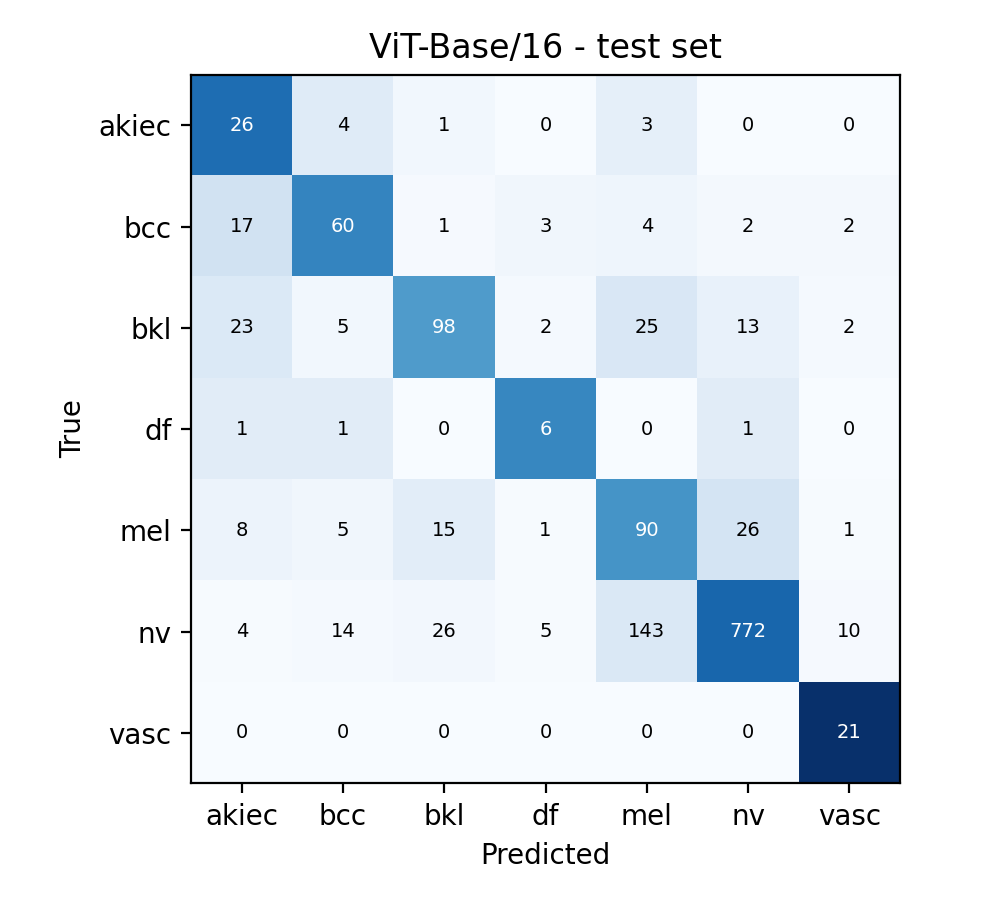
\includegraphics[width=0.42\textwidth]{results/vit_confusion_test.png}}{}
\caption{Test-set confusion matrices (counts; shading is row-normalised recall). Left: ResNet-50; right: ViT-Base.}
\label{fig:cm}
\end{figure*}

\section{Conclusion and limitations}
I fine-tuned ResNet-50 and ViT-Base on HAM10000 on a laptop GPU, with a lesion-level split, class-weighted loss and augmentation, and evaluated both on held-out lesions with imbalance-aware metrics (Section~\ref{sec:results}).
With this short training budget the two architectures reach similar balanced accuracy (\resnetTestBacc{} and \vitTestBacc{}), and the difference is within test-set noise; ResNet-50 trains about 2.6 times faster per epoch on the laptop GPU.
Both remain weak on melanoma, the most clinically important class.

The study has clear limitations.
It is a single run with one seed and one split, with only a few epochs and no hyperparameter search, so the comparison may change under a larger budget; Vision Transformers lack some of the inductive biases of CNNs and depend more on pre-training scale~\cite{dosovitskiy2021image}, so their relative standing is sensitive to these choices.
The rarest classes have few test images (9 for dermatofibroma, 21 for vascular lesions), so their recall estimates are noisy.
PyTorch's MPS backend is not fully deterministic, so a rerun can give slightly different numbers.
Finally, HAM10000 was collected at two sites and does not represent all skin types, imaging devices or clinical settings~\cite{tschandl2018ham10000}; test performance on its own held-out lesions says nothing about clinical use.

Natural next steps are repeating the run over several seeds, training longer at higher resolution, and evaluating on an external dataset.


\bibliographystyle{plain}
\bibliography{main}

\onecolumn
\appendix
\section{Explanation maps}

Figure~\ref{fig:maps} shows, for one test image of melanoma, basal cell carcinoma and nevus, which regions each fine-tuned model's prediction is sensitive to.
For ResNet-50 I use Grad-CAM~\cite{selvaraju2017gradcam} on the last convolutional block; for ViT-Base I use attention rollout~\cite{abnar2020quantifying}, which multiplies the head-averaged attention matrices of all layers (with the residual connection added) and reads off the attention from the class token to each patch.
Both maps are computed for the class the model predicts; they are produced by \texttt{scripts/visualize.py}.

These maps are qualitative.
The images are simply the first test image of each of the three classes, not chosen for how the maps look.
In all three, the ResNet-50 Grad-CAM map lies mostly on the lesion.
The ViT attention-rollout maps are more diffuse and also give high values to image corners and borders, including the ruler marks in the bottom-right corner of the melanoma image.
Three images cannot show whether this means ViT relies on such artefacts or is a property of attention rollout itself.
ViT misclassifies the basal cell carcinoma as melanoma with low confidence (0.29), whereas ResNet-50 classifies it correctly.
None of this demonstrates that either model relies on clinically meaningful features.

\begin{figure}[h]
\centering
\IfFileExists{supplementary/attention_map.png}{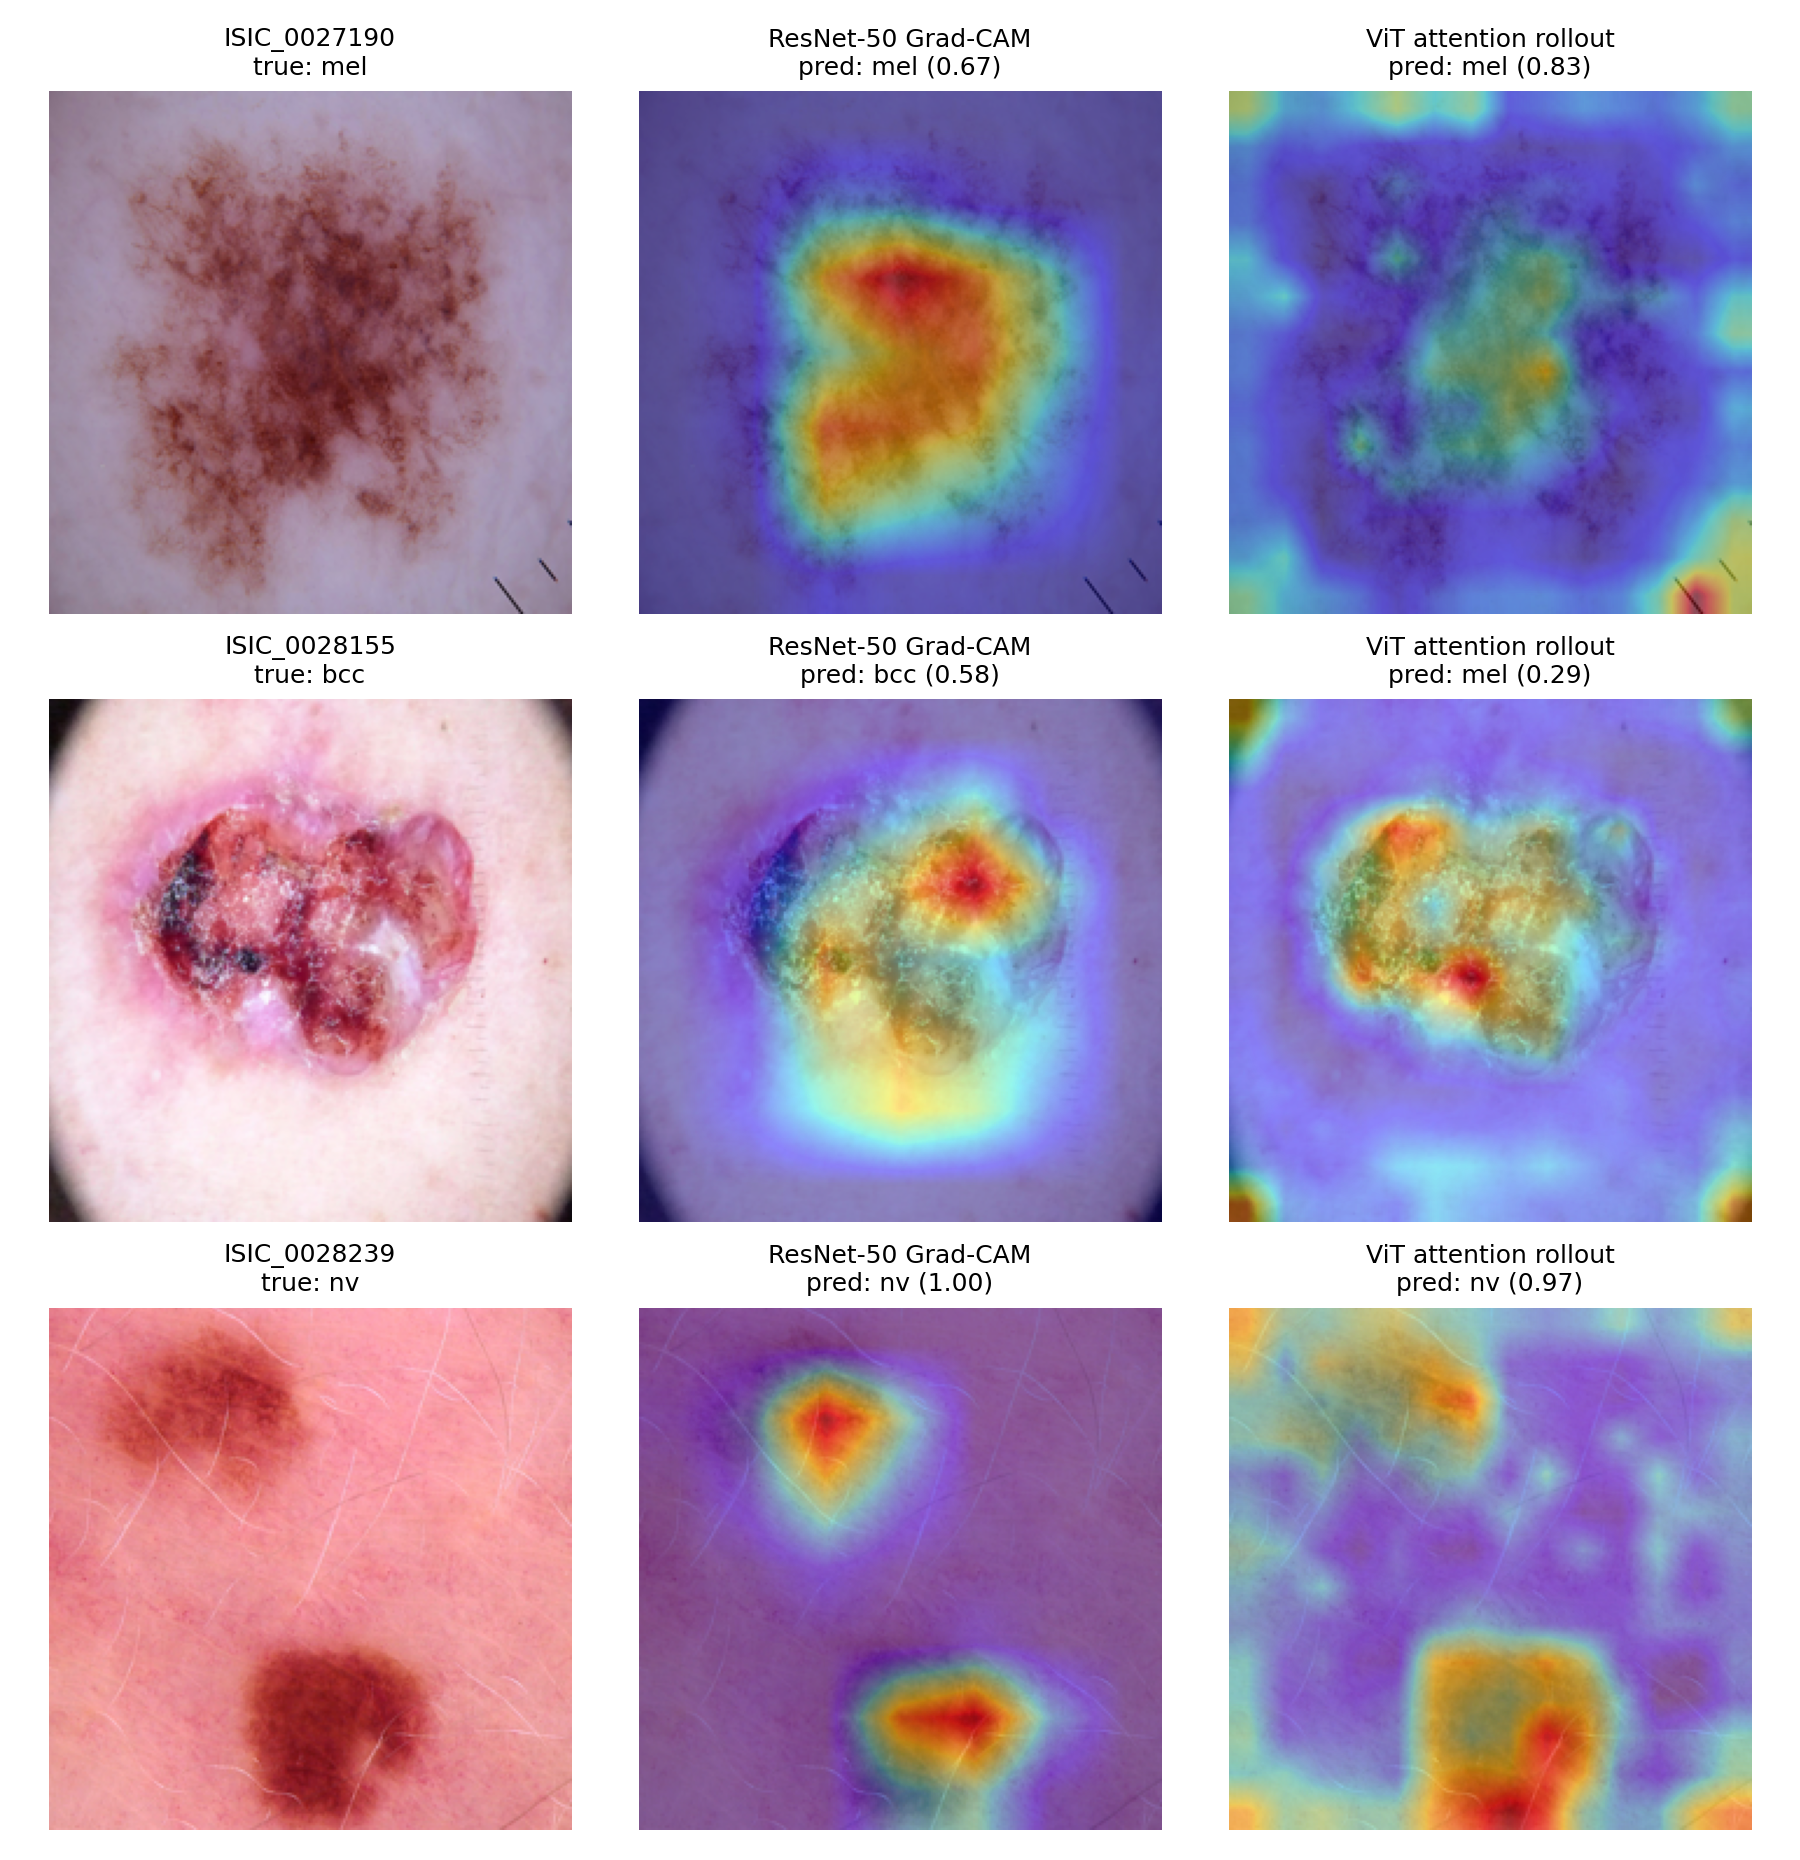
\includegraphics[width=0.62\textwidth]{supplementary/attention_map.png}}{\textit{Run scripts/visualize.py to generate this figure.}}
\caption{Left: test image with its true label. Middle: ResNet-50 Grad-CAM. Right: ViT-Base attention rollout. Titles give each model's prediction and softmax confidence.}
\label{fig:maps}
\end{figure}


\end{document}
